\documentclass[herrin-thesis.tex]{subfiles}
\begin{document}

\chapter{Neutrinos}
\label{ch:neutrinos}

\section{History}
\subsection{Beta Decay}
Neutrino physics first arose in the study of beta decay. In the most basic form of beta decay, a neutron in the nucleus decays to a proton and emits an electron. \todo{Who first found a continuous spectrum for the electron?}Early nuclear physicists discovered that unlike alpha particles and gamma rays, which are emitted in monoenergetic lines from nuclear processes, beta decay electrons were emitted with a continuous range of energies. Rather than abandoning the principle of energy conservation, Wolfgang Pauli\addref in 1930 proposed a massless particle that could carry away the ``missing energy'' in beta decays. In 1933, Enrico Fermi\addref combined the idea with Heisenberg's nucleon model to form a theory of beta decay.

\subsection{Discovery}
For several decades after Pauli proposed the neutrino, the only evidence for its existence was indirect, through momentum and energy conservation. It was not until 1956 that Cowan and Reines\addref observed the electron antineutrino. Their experiment consisted of a large tank of water with cadmium chloride dissolved. Electron antineutrinos from a nearby nuclear reactor would interact with protons in the water molecules, creating a positron and a neutron. In the experiment, the positron annihilated, producing gamma rays. Cadmium is a good neutron absorbed, and the capture created another gamma ray. The delayed coincidence of the two gamma rays provided evidence of inverse beta decay.

The discovery of the muon in 1936 provided the possibility of a muon neutrino, distinct from the electron neutrino. In 1962, Lederman, Schwartz, and Steinberger\addref showed that a beam of neutrinos, created from a beam of decaying pions, aways interacted to form muons and not electrons. We now know that each charged lepton forms an isospin doublet with its associated neutrino.

\subsection{The Solar Neutrino Problem}

\section{The Nature of the Neutrino}

\section{Neutrino Mixing and Oscillation}
Neutrino mixing is described by the unitary Pontecorco-Maki-Nakagawa-Sakata (PMNS) matrix \(U\). In the case of three mass eigenstates and 3 flavor eigenstates, \(U\) can be parameterized by three Euler rotation angles, one Dirac CP violation phase, and two Majorana CP violation phases (is the neutrino is a Majorana particle):
\begin{align}
U =&\begin{pmatrix}
	U_{e1}	&	U_{e2}	& 	U_{e3}	\\
	U_{\mu1}	&	U_{\mu2}	& 	U_{\mu3}	\\
	U_{\tau1}	&	U_{\tau2}	& 	U_{\tau3}	\\
	\end{pmatrix}\\
%     =&\begin{pmatrix}
%	1	&	0		&	0		\\
%	0	&	c_{23}	&	s_{23}	\\
%	0	&	-s_{23}	&	c_{23}	\\
%	\end{pmatrix}
%	\begin{pmatrix}
%	c_{13}			&	0	&	s_{13}e^{-i\delta}	\\
%	0				&	1	&	0				\\
%	-s_{13}e^{i\delta}	&	0	&	c_{13}			\\
%	\end{pmatrix}
%	\begin{pmatrix}
%	c_{12}	&	s_{12}	&	0	\\
%	-s_{12}	&	c_{12}	&	0	\\
%	0		&	0		&	1	\\
%	\end{pmatrix}
	=&\begin{pmatrix}
	c_{12}c_{13}							&	s_{12}c_{13}							&	s_{13}e^{-i\delta}	\\
	-s_{12}c_{23}-c_{12}s_{23}s_{13}e^{i\delta}	&	c_{12}c_{23}-s_{12}s_{23}s_{13}e^{i\delta}	&	s_{23}c_{13}		\\
	s_{12}s_{23}-c_{12}c_{23}s_{13}e^{i\delta}	&	-c_{12}s_{23}-s_{12}c_{23}s_{13}e^{i\delta}	&	c_{23}c_{13}
	\end{pmatrix}
	\begin{pmatrix}
	1	&	0					&	0	\\
	0	&	e^{\frac{i\alpha_{21}}{2}}	&	0	\\
	0	&	0					&	e^{\frac{i\alpha_{31}}{2}}
	\end{pmatrix}\nonumber
\label{eq:nu_pmns_matrix}
\end{align}
where the \(s_{ij}\) denote \(\sin\theta_{ij}\) and \(c_{ij}\) denote \(\cos\theta_{ij}\). \(\delta\) is the Dirac CP violation phase, and \(\alpha_{21}\) and \(\alpha_{31}\) are the Majorana CP violation phases.

 A flavor eigenstate, such as a neutrino produced by the decay of a lepton, is a superposition of mass eigenstates:
 \begin{equation}
 \Ket{\nu_{\ell}} = \sum_{i}U_{\ell i}^{*} \Ket{\nu_i}
 \label{eq:nu_superposition}
 \end{equation}
 This mixing is illustrated in \cref{fig:nu_mixing}.
 
 The time evolution of a mass eigenstate is simply
 \begin{equation}
 \Ket{\nu_{i}(t)} = e^{-i(E_i t - \vec{p}_i\cdot\vec{x})}\Ket{\nu_i(0)}
 \label{eq:nu_time_evolution}
 \end{equation}

Neutrinos have such small masses that they are always observed in a hyper-relativistic state, in which \(t\approx L\), \(p\approx E\), where \(E\) is the total energy of the neutrino. In this limit, the phase in the exponent for \cref{eq:nu_time_evolution} becomes \(m_i^2 L/(2E)\). Combining this and \cref{eq:nu_superposition}, then the probability for a neutrino with flavor \(\alpha\) and energy \(E\) to oscillate to a neutrino with flavor \(\beta\) after traveling distance \(L\) is
\begin{align}
P_{\alpha\rightarrow\beta}	& = \left | \Braket{\nu_\beta | \nu_\alpha(L)} \right |	& = \delta_{\alpha\beta}	& - 4\sum_{i>j}\text{Re}\left(U_{\alpha i}^{*}U_{\beta i}U_{\alpha j}U_{\beta j}^{*}\right)\sin^2\left(\frac{\Delta m_{ij}^2 L}{4 E}\right)\nonumber\\
						&										&					& +2\sum_{i>j}\text{Im}\left(U_{\alpha i}^{*}U_{\beta i}U_{\alpha j}U_{\beta j}^{*}\right)\sin^2\left(\frac{\Delta m_{ij}^2 L}{2 E}\right)
\label{eq::nu_oscillation_prob}
\end{align}
Thus, the probability depends only on the angles in the mixing matrix \(U\), the difference between the squares of the masses \(\Delta m_{ij}^2\), and the ratio of distance travelled to neutrino energy \(L/E\). If there is no Dirac CP phase, \(U\) is real and the second sum is zero. Since the Majorana phases only enter \(U\) as a diagonal factor, they do not affect the oscillation probability, and thus oscillation experiments cannot determine the Majorana nature of the neutrino.

\section{Massive Neutrinos}

\begin{figure}
	\centering
	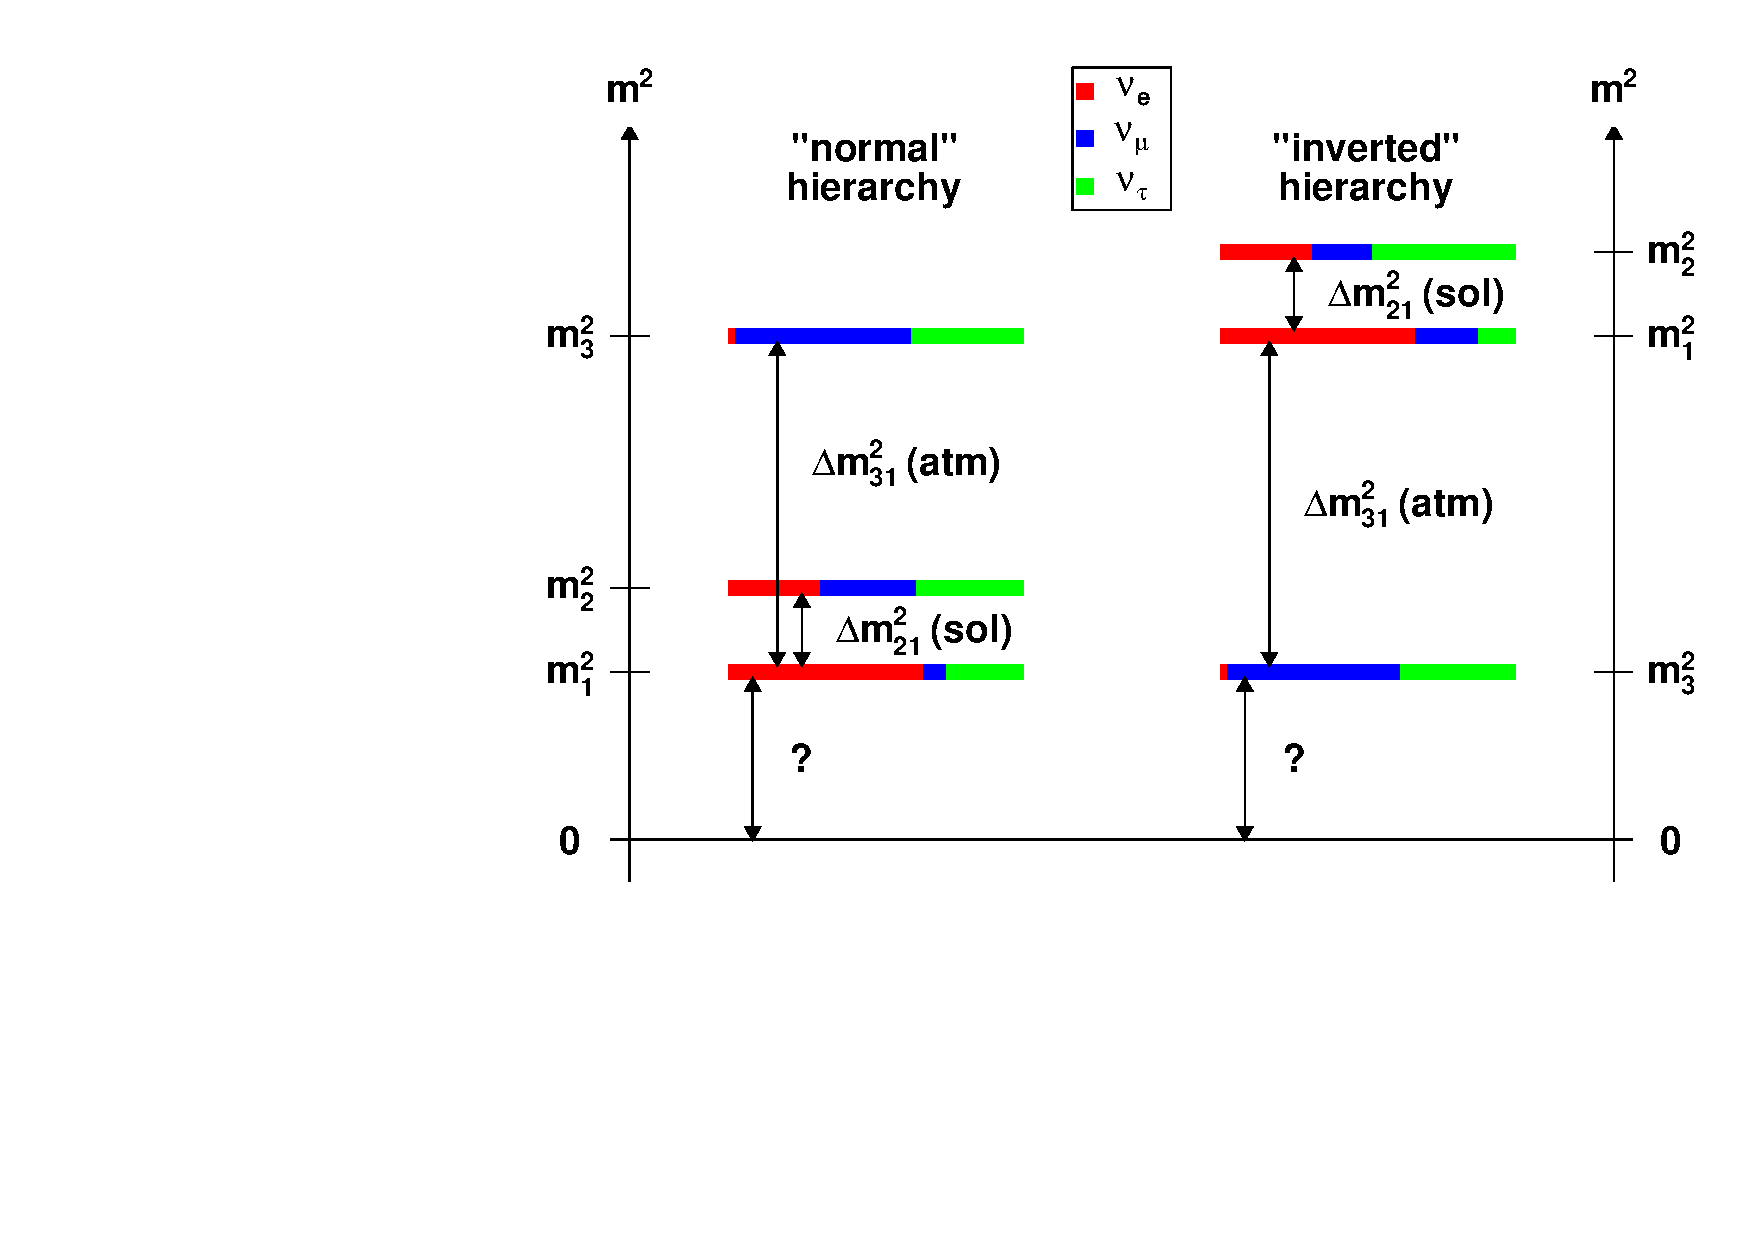
\includegraphics[width=0.6\textwidth]{./plots/nu_mixing.pdf}
	\caption[Neutrino mixing]{The neutrino mass eigenstates (represented by the horizontal bands) are each a mixture of the flavor eigenstates (represented by the different colors). The mixing angles in the PMNS matrix provide the flavor compositions of each mass state. The splittings between the squares of the masses of the mass eigenstates are known (but not shown to scale), though the sign of \(\Delta m_{31}^2\) remains unknown, allowing for the possibility of an ``inverted'' mass hierarchy. The absolute scale of the neutrino masses is also unknown.}
	\label{fig:nu_mixing}
\end{figure}

Neutrinos are observed to oscillate, and thus according to \cref{eq:nu_oscillation_prob}, the mass-squared splittings have been measured to be nonzero. The sign of \(\Delta m_{21}\) is known from the effect of matter on neutrinos emitted by the sun (known as the MSW effect), while only the magnitude of \(\Delta m_{31}\) is known. The mass splittings provide a weak lower bounds on the masses of two mass eigenstates. This does not determine the absolute mass scale, however, and the lightest eigenstate may have zero mass. If also does not determine which mass eigenstate is the lightest. \Cref{fig:nu_mixing} summarizes the situation. Other experiments, described below, may be able to measure the absolute mass scale and possibly determine the hierarchy of the mass eigenstates. However, to date, they have only provided upper bounds on the mass.

\begin{figure}
	\centering
	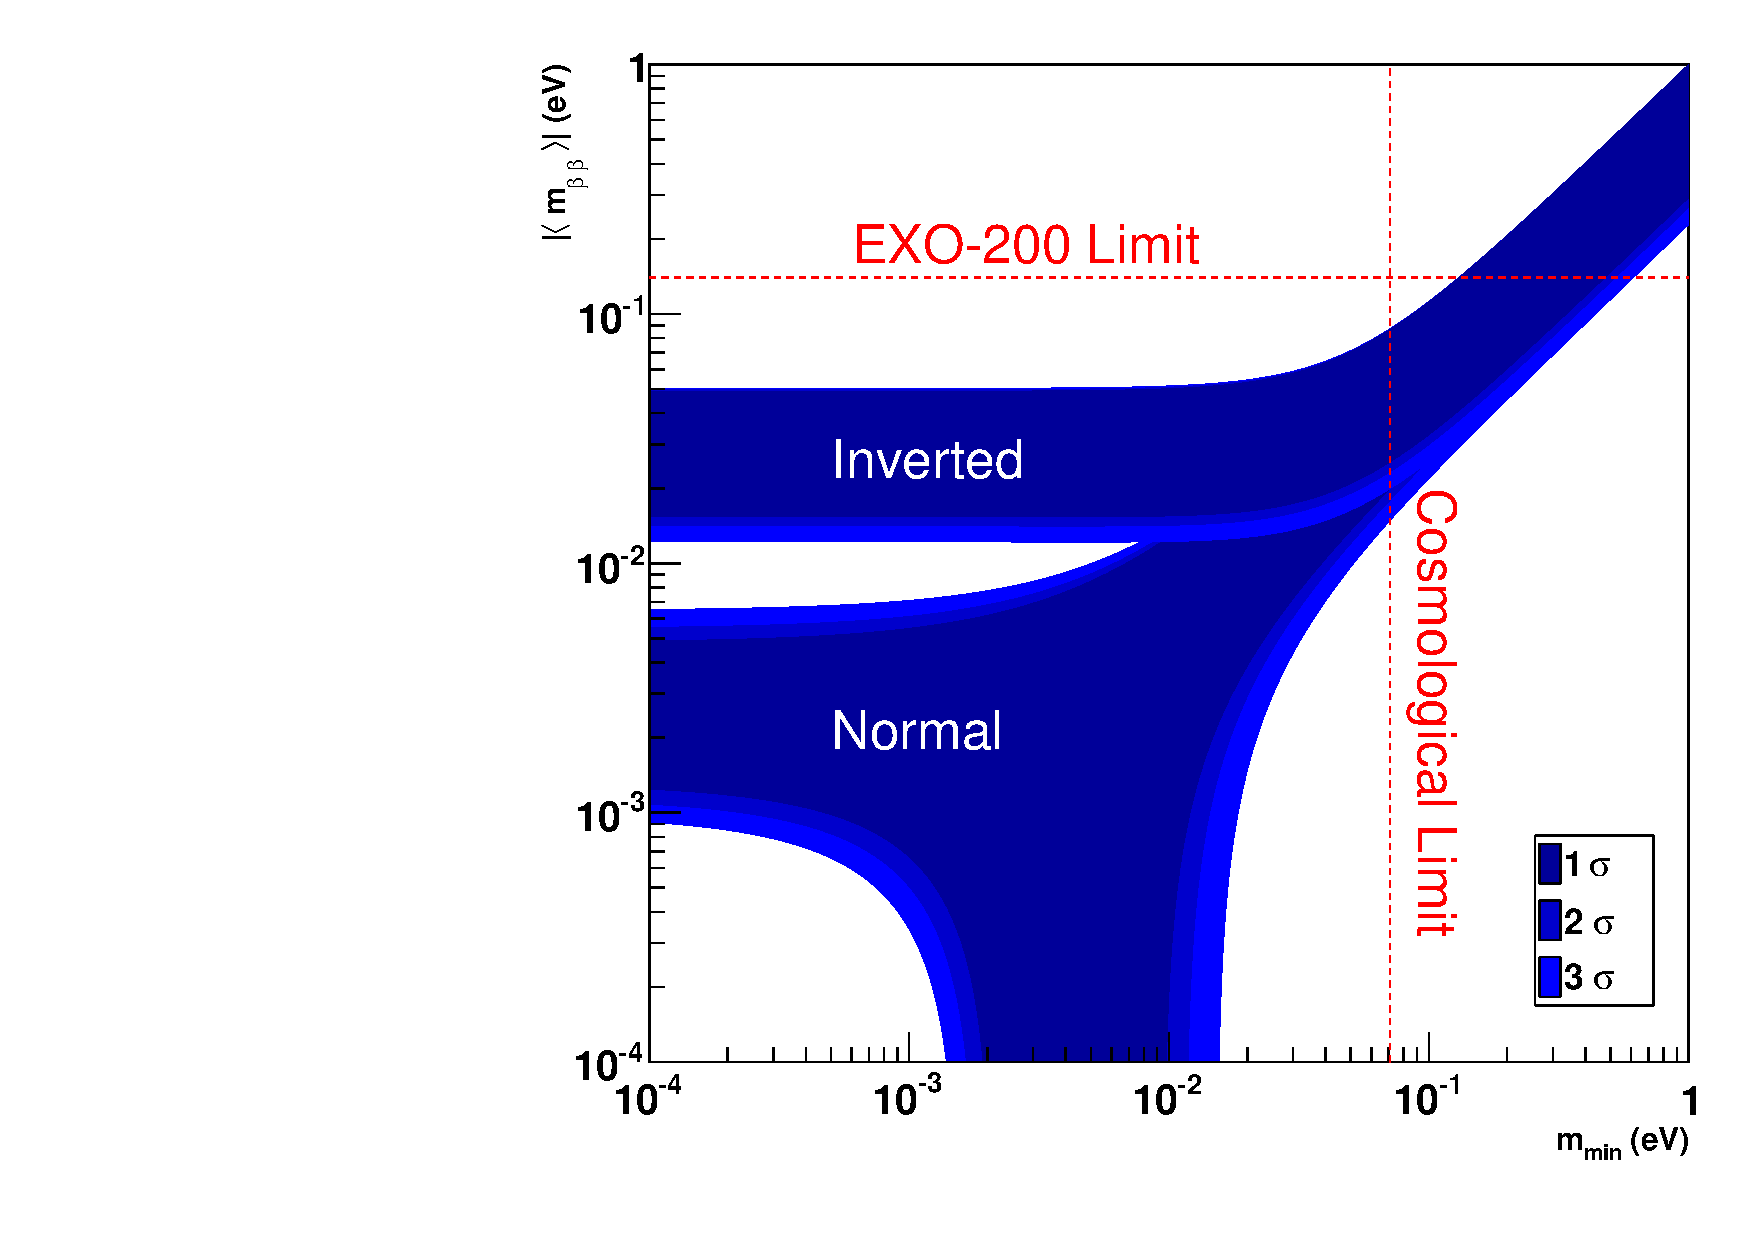
\includegraphics[width=0.6\textwidth]{./plots/nu_meff_v_mmin.pdf}
	\caption[Effective Majorana mass vs. smallest neutrino mass]{The allowed values for the effective Majorana mass as a function of the smallest neutrino mass for both the inverted and normal mass hierarchies. The widths of the bands depend on the Majorana phases. Uncertainties on the mixing angles and mass splittings widen these bands.The mixing angles, mass splittings, and uncertainties used are from a global fit by Forero et al.\cite{Forero:2012cr} The cosmological limit comes from the Planck satellite. Constraints on the sum of the neutrino masses combined with the mass splittings yield an upper bound for the smallest neutrino mass.}
	\label{fig:nu_meff_v_mmin}
\end{figure}\addref

\subsection{Beta Decay Endpoint}

\subsection{Majorana Particles}

\subsection{Double Beta Decay}

\begin{figure}
	\centering
	\begin{subfigure}[b]{0.48\textwidth}
		\centering
		\includegraphics[width=\textwidth]{./feynman_diagrams/twonubetabeta.pdf}
		\caption[Diagram of \(2\nu\beta\beta\)]{The standard model allowed mode of two neutrino double beta decay.}
		\label{fig:diagram_2nubb}
	\end{subfigure}\hfill%
         \begin{subfigure}[b]{0.48\textwidth}
		\centering
		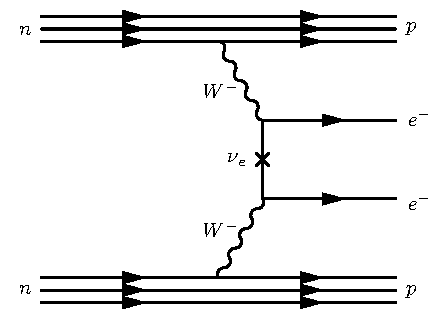
\includegraphics[width=\textwidth]{./feynman_diagrams/zeronubetabeta.pdf}
		\caption[Diagram of \(0\nu\beta\beta\)]{The neutrinoless mode of double beta decay.}
		\label{fig:diagram_0nubb}
	\end{subfigure}
	\label{fig:diagrams}
	\caption[Double beta decay modes]{Double beta decay modes}
\end{figure}

\end{document}